\documentclass[11pt,a4paper]{article}

% Required packages
\usepackage{graphicx}
\usepackage{xcolor}
\usepackage{geometry}
\usepackage{amsmath}
\usepackage{amssymb}
\usepackage{amsthm}
\usepackage{booktabs}
\usepackage{array}
\usepackage{enumitem}
\usepackage{fancyhdr}
\usepackage{titlesec}
\usepackage{setspace}
\usepackage{microtype}
\usepackage{parskip}
\usepackage{tcolorbox}
\usepackage{tikz}

% Page geometry
\geometry{a4paper, top=2.5cm, bottom=2.5cm, left=3cm, right=2.5cm}

% Line spacing
\onehalfspacing

% Define colors
\definecolor{darkblue}{RGB}{26,26,46}
\definecolor{accentblue}{RGB}{15,52,96}
\definecolor{theoremcolor}{RGB}{50,50,50}

% Theorem environments
\theoremstyle{definition}
\newtheorem{definition}{Definition}[section]
\newtheorem{theorem}{Theorem}[section]

% tcolorbox settings
\tcbuselibrary{skins,breakable}

% Header and footer
\pagestyle{fancy}
\fancyhf{}
\fancyhead[C]{\small\itshape An Investigation into Turing Machines}
\fancyfoot[C]{\thepage}
\renewcommand{\headrulewidth}{0.4pt}

% Section formatting
\titleformat{\section}{\Large\bfseries}{\thesection.}{0.5em}{}
\titleformat{\subsection}{\large\bfseries}{\thesubsection}{0.5em}{}

% hyperref - MUST load last
\usepackage[
    colorlinks=true,
    linkcolor=blue,
    citecolor=darkgray,
    urlcolor=blue,
    bookmarks=true,
    bookmarksnumbered=true,
    unicode=true,
    pdftitle={An Investigation into Turing Machines},
    pdfauthor={Academic Research},
    pdfsubject={Computational Theory},
    pdfkeywords={Turing machine, computability, Church-Turing thesis, halting problem}
]{hyperref}

\begin{document}

% Title page
\begin{titlepage}
\begin{tikzpicture}[remember picture,overlay]
    \fill[darkblue] (current page.south west) rectangle (current page.north east);
    % Geometric decorations
    \fill[accentblue,opacity=0.5] (current page.north west) circle (8cm);
    \fill[accentblue,opacity=0.3] ([xshift=3cm,yshift=-5cm]current page.north east) circle (6cm);
    \draw[white,opacity=0.2,line width=1pt] ([yshift=-4cm]current page.north west) -- ([yshift=-4cm]current page.north east);
    % Tape decoration
    \draw[white,opacity=0.3] (-3,3) rectangle ++(1.2,1.5);
    \node[white,opacity=0.7] at (-2.4,3.75) {\texttt{0}};
    \draw[white,opacity=0.3] (-1.5,3) rectangle ++(1.2,1.5);
    \node[white,opacity=0.7] at (-0.9,3.75) {\texttt{1}};
    \draw[red!60,line width=2pt] (0,3) rectangle ++(1.2,1.5);
    \node[white] at (0.6,3.75) {\texttt{1}};
    \draw[white,opacity=0.3] (1.5,3) rectangle ++(1.2,1.5);
    \node[white,opacity=0.7] at (2.1,3.75) {\texttt{0}};
    \draw[white,opacity=0.3] (3,3) rectangle ++(1.2,1.5);
    \node[white,opacity=0.7] at (3.6,3.75) {\texttt{1}};
    \draw[white,opacity=0.3] (4.5,3) rectangle ++(1.2,1.5);
    \node[white,opacity=0.7] at (5.1,3.75) {\texttt{B}};
\end{tikzpicture}

\vspace*{8cm}
\begin{center}
    {\Huge\bfseries\color{white} An Investigation into\\[0.3cm] Turing Machines}\\[1cm]
    {\Large\color{white!80}\itshape Foundations of Computational Theory and\\the Limits of Algorithmic Computation}\\[3cm]
    {\large\color{white}
    Academic Paper\\[0.3cm]
    Department of Computer Science\\[0.3cm]
    February 2026
    }
\end{center}
\end{titlepage}

% Abstract
\thispagestyle{empty}
\begin{abstract}
\noindent The Turing machine, introduced by Alan Turing in 1936, stands as one of the most fundamental constructs in theoretical computer science. This paper provides a comprehensive investigation into Turing machines, examining their historical origins, formal mathematical definition, and profound implications for the theory of computation. We explore the Church-Turing thesis, which posits that Turing machines capture the intuitive notion of effective computability, and analyze the halting problem as a demonstration of the inherent limits of algorithmic computation. The paper further discusses universal Turing machines, the relationship between Turing machines and modern computers, and the continuing significance of this theoretical framework in contemporary computer science research. Through this investigation, we demonstrate that despite being conceived nearly ninety years ago, the Turing machine remains the cornerstone of our understanding of what can and cannot be computed.

\vspace{0.5cm}
\noindent\textbf{Keywords:} Turing machine, computability theory, Church-Turing thesis, halting problem, universal computation, decidability, algorithmic complexity
\end{abstract}

\newpage
\tableofcontents
\newpage

\section{Introduction}\label{sec:intro}

The concept of the Turing machine represents one of the most significant intellectual achievements in the history of mathematics and computer science. Introduced by the British mathematician Alan Turing in his seminal 1936 paper ``On Computable Numbers, with an Application to the Entscheidungsproblem,'' the Turing machine was designed as a theoretical model to formalize the intuitive notion of algorithmic computation. Despite its apparent simplicity---consisting merely of an infinite tape, a read-write head, and a finite set of states---the Turing machine has proven capable of expressing any computation that can be performed by any modern computer.

The significance of Turing's work extends far beyond the abstract realm of mathematical logic. The Turing machine provides the theoretical foundation for understanding the capabilities and limitations of digital computers. It establishes a precise boundary between problems that can be solved algorithmically and those that cannot, thereby defining the very nature of computation itself. As Hodges noted in his comprehensive biography of Turing, the construction provided ``an argument from first principles'' that demonstrated what mechanical computation could achieve.

This paper aims to provide a thorough investigation into Turing machines, examining their historical origins, mathematical formalization, and theoretical implications. We begin by exploring the intellectual context in which Turing developed his ideas, then proceed to the formal definition of Turing machines. Subsequently, we analyze the Church-Turing thesis, which asserts the equivalence between Turing computability and effective calculability. The paper culminates with a discussion of the halting problem, which demonstrates fundamental limits on what can be computed, and examines the relationship between Turing machines and contemporary computing systems.

\section{Historical Background}\label{sec:history}

\subsection{The Entscheidungsproblem}

The development of the Turing machine was motivated by one of the great challenges of early twentieth-century mathematics: the \emph{Entscheidungsproblem}, or ``decision problem.'' This problem was posed by David Hilbert and Wilhelm Ackermann in 1928 and asked whether there exists a general algorithmic procedure that could determine, for any statement in first-order logic, whether that statement is provable. The problem was central to Hilbert's program of establishing the foundations of mathematics on a firm, decidable basis.

Before Turing's work, the notion of an ``effective procedure'' or ``algorithm'' remained informal and intuitive. Mathematicians understood algorithms as step-by-step procedures that could, in principle, be carried out by a human following explicit instructions. However, there was no rigorous mathematical definition that could be used to prove whether such procedures existed for particular problems. This lacuna presented a significant obstacle to resolving the Entscheidungsproblem, as any answer required first establishing what constituted an effective method of computation.

\subsection{Concurrent Developments}

Turing was not alone in seeking to formalize the notion of effective computability. Around the same time, Alonzo Church at Princeton University developed the lambda calculus as an alternative formalization. Church used this formalism to prove that the Entscheidungsproblem had no solution, publishing his result shortly before Turing's paper appeared. Stephen Kleene and J.B. Rosser, working with Church, developed the theory of recursive functions as yet another equivalent formalization.

Emil Post independently proposed a formalism remarkably similar to Turing's machines in 1936. Post's ``worker'' model described a human moving from room to room, writing and erasing marks according to a list of instructions. However, Post presented this as a definition of solvability rather than proving theorems about uncomputability, and his work appeared in a shorter, less developed form than Turing's comprehensive analysis.

What distinguished Turing's approach was its directness and intuitive appeal. Church himself recognized that Turing's analysis made ``the identification with effectiveness in the ordinary (not explicitly defined) sense evident immediately.'' The Turing machine model, with its concrete imagery of a tape and read-write head, provided an immediately comprehensible model of mechanical computation that could be understood without specialized mathematical training.

\section{Formal Definition of Turing Machines}\label{sec:formal}

\subsection{Intuitive Description}

A Turing machine can be visualized as a device operating on an infinite tape divided into discrete cells. Each cell contains a symbol from a finite alphabet. A read-write head is positioned over one cell at any given time and can read the symbol in that cell, write a new symbol, and move one cell to the left or right. The machine operates according to a finite set of rules that determine, based on the current state and the symbol being read, what action to take.

\begin{figure}[htbp]
\centering
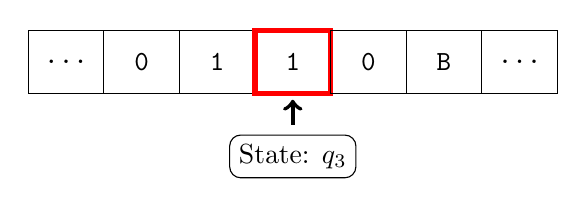
\begin{tikzpicture}[scale=0.8]
    % Tape cells
    \draw (0,0) rectangle ++(1.2,1); \node at (0.6,0.5) {\texttt{...}};
    \draw (1.2,0) rectangle ++(1.2,1); \node at (1.8,0.5) {\texttt{0}};
    \draw (2.4,0) rectangle ++(1.2,1); \node at (3.0,0.5) {\texttt{1}};
    \draw[red,line width=2pt] (3.6,0) rectangle ++(1.2,1); \node at (4.2,0.5) {\texttt{1}};
    \draw (4.8,0) rectangle ++(1.2,1); \node at (5.4,0.5) {\texttt{0}};
    \draw (6.0,0) rectangle ++(1.2,1); \node at (6.6,0.5) {\texttt{B}};
    \draw (7.2,0) rectangle ++(1.2,1); \node at (7.8,0.5) {\texttt{...}};
    % Read-write head
    \draw[->,line width=1.5pt] (4.2,-0.5) -- (4.2,-0.1);
    \node[draw,rounded corners] at (4.2,-1) {State: $q_3$};
\end{tikzpicture}
\caption{Schematic representation of a Turing machine. The tape extends infinitely in both directions, with the read-write head positioned over the current cell (highlighted).}\label{fig:tm-schema}
\end{figure}

\subsection{Mathematical Formalization}

Following the standard definition presented by Hopcroft and Ullman, a Turing machine is formally defined as a 7-tuple:

\begin{definition}[Turing Machine]\label{def:tm}
A Turing machine is a 7-tuple $M = (Q, \Sigma, \Gamma, \delta, q_0, B, F)$ where:
\begin{itemize}[itemsep=0.2em]
    \item $Q$ is a finite set of states
    \item $\Sigma$ is the input alphabet (not containing the blank symbol)
    \item $\Gamma$ is the tape alphabet, where $\Sigma \subseteq \Gamma$
    \item $\delta: Q \times \Gamma \rightarrow Q \times \Gamma \times \{L, R\}$ is the transition function
    \item $q_0 \in Q$ is the initial state
    \item $B \in \Gamma \setminus \Sigma$ is the blank symbol
    \item $F \subseteq Q$ is the set of accepting (final) states
\end{itemize}
\end{definition}

The transition function $\delta$ encodes the machine's behavior. Given the current state $q$ and the symbol $a$ currently under the read-write head, $\delta(q, a) = (q', b, D)$ specifies that the machine should:
\begin{enumerate}
    \item Transition to state $q'$
    \item Write symbol $b$ in the current cell (replacing $a$)
    \item Move the head in direction $D$, where $L$ denotes left and $R$ denotes right
\end{enumerate}

\subsection{Configuration and Computation}

A configuration of a Turing machine captures its complete state at any point during computation. Formally, a configuration is a triple $(q, \alpha, i)$ where $q$ is the current state, $\alpha$ is the tape contents (represented as a string over $\Gamma$), and $i$ is the position of the read-write head.

A computation is a sequence of configurations $C_0, C_1, C_2, \ldots$ where each $C_{i+1}$ follows from $C_i$ according to the transition function $\delta$. The machine accepts an input if the computation reaches a configuration with a state in $F$. The machine rejects if it reaches a configuration from which no transition is defined and the current state is not in $F$.

\subsection{Example: Binary Addition}

To illustrate how Turing machines operate, consider a simple machine that adds 1 to a binary number. The input is a binary string, and the output should be the binary representation of the original number plus one.

\begin{table}[htbp]
\centering
\caption{Transition table for a Turing machine that adds 1 to a binary number}\label{tab:binary-add}
\begin{tabular}{@{}ccccc@{}}
\toprule
Current State & Read & Write & Move & Next State \\
\midrule
$q_0$ & 0 & 0 & R & $q_0$ \\
$q_0$ & 1 & 1 & R & $q_0$ \\
$q_0$ & B & B & L & $q_1$ \\
$q_1$ & 0 & 1 & L & $q_2$ \\
$q_1$ & 1 & 0 & L & $q_1$ \\
$q_1$ & B & 1 & L & $q_2$ \\
$q_2$ & 0 & 0 & L & $q_2$ \\
$q_2$ & 1 & 1 & L & $q_2$ \\
$q_2$ & B & B & R & $q_f$ \\
\bottomrule
\end{tabular}
\end{table}

The machine operates in three phases: in state $q_0$, it scans right to find the end of the input; in state $q_1$, it performs the addition by carrying as necessary; in state $q_2$, it returns to the beginning of the result before halting in the accept state $q_f$.

\section{The Church-Turing Thesis}\label{sec:thesis}

\subsection{Statement of the Thesis}

The Church-Turing thesis represents one of the most important and enduring claims in the foundations of computer science. It asserts that any function that can be computed by what we intuitively understand as an ``algorithm'' or ``effective procedure'' can be computed by a Turing machine. Conversely, any function computable by a Turing machine represents a valid algorithmic computation.

\begin{tcolorbox}[colback=gray!5,colframe=theoremcolor,title=Church-Turing Thesis]
\textit{A function on the natural numbers is effectively calculable if and only if it is computable by a Turing machine.}
\end{tcolorbox}

It is crucial to understand that the Church-Turing thesis is not a mathematical theorem but rather a thesis or hypothesis. It cannot be proved because it relates a formal mathematical concept (Turing computability) to an informal intuitive concept (effective calculability). As Kleene observed, ``the thesis has the character of an hypothesis---a point emphasized by Post and by Church.''

\subsection{Evidence for the Thesis}

Despite its unprovable nature, the Church-Turing thesis is supported by overwhelming evidence. Multiple independent formalizations of computability---including Turing machines, the lambda calculus, recursive functions, Post production systems, and register machines---have all been proven equivalent. Every proposed model of computation has either been shown equivalent to Turing machines or demonstrably weaker.

\begin{theorem}[Rosser, 1939]\label{thm:rosser}
The following classes of functions are coextensive:
\begin{enumerate}
    \item The lambda-definable functions
    \item The general recursive functions
    \item The Turing-computable functions
\end{enumerate}
\end{theorem}

In subsequent decades, many additional computational models were shown to be Turing-equivalent. Hao Wang and Martin Davis simplified Turing machines into what is now known as the Post-Turing machine. Marvin Minsky developed multi-tape machines and counter machines. Stephen Kleene's register machines anticipated the architecture of modern computers. In every case, the computational power remained identical to that of the original Turing machine.

\subsection{Implications and Interpretations}

The Church-Turing thesis has profound implications for computer science and mathematics. It establishes that there exists a universal notion of computability independent of any particular formalism or machine architecture. This universality means that results proved for Turing machines---including both positive results about what can be computed and negative results about what cannot---apply to all reasonable models of computation.

Different interpretations of the thesis have been proposed. Church viewed the identification as a definition, while Post considered it a natural law subject to potential empirical refutation. Modern axiomatic approaches, such as those developed by Sieg and by Dershowitz and Gurevich, attempt to derive the thesis from more fundamental principles.

\section{The Halting Problem and Undecidability}\label{sec:halting}

\subsection{Statement of the Problem}

Perhaps the most celebrated result concerning Turing machines is the undecidability of the halting problem. This problem asks whether there exists an algorithm that, given a description of a Turing machine and an input, can determine whether that machine will eventually halt on that input or run forever.

\begin{definition}[Halting Problem]\label{def:halting}
The halting problem is the decision problem: given a Turing machine $T$ and an input $w$, determine whether $T$ halts when run on input $w$.
\end{definition}

Turing proved that no Turing machine can solve this problem in general. This result demonstrates a fundamental limitation on algorithmic computation---there exist well-defined questions that no algorithm can answer.

\subsection{Proof of Undecidability}

The proof proceeds by contradiction using a diagonalization argument reminiscent of Cantor's proof that the real numbers are uncountable.

\begin{theorem}[Turing, 1936]\label{thm:halting}
The halting problem is undecidable. That is, there exists no Turing machine that, given any Turing machine $T$ and input $w$, correctly determines whether $T$ halts on $w$.
\end{theorem}

\begin{proof}
Assume, for contradiction, that there exists a Turing machine $H$ that solves the halting problem. That is, for any machine $T$ and input $w$:
\begin{equation}\label{eq:halt}
H(T, w) = \begin{cases} \text{HALT} & \text{if } T \text{ halts on } w \\ \text{LOOP} & \text{if } T \text{ does not halt on } w \end{cases}
\end{equation}

We construct a new machine $D$ that, given a machine description $T$ as input:
\begin{enumerate}
    \item Runs $H(T, T)$ to determine if $T$ halts when given its own description as input
    \item If $H$ outputs HALT, then $D$ enters an infinite loop
    \item If $H$ outputs LOOP, then $D$ halts
\end{enumerate}

Now consider what happens when we run $D$ on its own description, $D(D)$:
\begin{itemize}
    \item If $D(D)$ halts, then by construction, $H(D, D)$ must have returned LOOP, meaning $D$ does not halt on $D$. Contradiction.
    \item If $D(D)$ does not halt, then $H(D, D)$ must have returned HALT, meaning $D$ halts on $D$. Contradiction.
\end{itemize}

In either case, we reach a contradiction. Therefore, our assumption that $H$ exists must be false, and no such halting-problem solver can exist.
\end{proof}

\subsection{Implications}

The undecidability of the halting problem has far-reaching consequences. It implies that there can be no general algorithm for proving program termination, no complete automatic verification of arbitrary programs, and no solution to Hilbert's Entscheidungsproblem. Together with Gödel's incompleteness theorems, it demolished Hilbert's program of finding a complete, decidable foundation for mathematics.

Many other problems have since been shown undecidable by reduction from the halting problem. These include: determining whether two context-free grammars generate the same language, the Post correspondence problem, Rice's theorem (stating that all non-trivial semantic properties of programs are undecidable), and countless problems in logic, algebra, and topology.

\section{Universal Turing Machines}\label{sec:universal}

\subsection{The Concept of Universality}

One of Turing's most profound insights was the existence of a universal Turing machine---a single machine capable of simulating any other Turing machine. Given an encoding of a Turing machine $T$ and an input $w$, the universal machine $U$ produces the same output that $T$ would produce on $w$.

\begin{definition}[Universal Turing Machine]\label{def:utm}
A universal Turing machine $U$ is a Turing machine such that for any Turing machine $T$ and input $w$, $U(\langle T \rangle, w) = T(w)$, where $\langle T \rangle$ denotes an encoding of $T$.
\end{definition}

The universal Turing machine embodies the principle that a single, fixed machine can perform any computation---the machine's behavior is determined entirely by its input, which includes both a program and data. This insight anticipated the stored-program computer architecture developed by John von Neumann a decade later.

\subsection{Construction}

To construct a universal machine, we must first establish an encoding scheme for Turing machines. Each state, symbol, and direction can be assigned a unique number, and the entire transition function can be encoded as a string of these numbers. The universal machine then operates as follows:
\begin{enumerate}
    \item Read and parse the encoded description of $T$
    \item Maintain a simulation of $T$'s tape and current state
    \item Look up the appropriate transition in $T$'s encoded transition table
    \item Apply the transition to the simulated configuration
    \item Repeat until $T$ halts (if ever)
\end{enumerate}

The technical details of this construction are intricate but the conceptual framework is straightforward: the universal machine acts as an interpreter, executing the program encoded in its input.

\section{Turing Machines and Modern Computation}\label{sec:modern}

\subsection{Relationship to Physical Computers}

Every modern digital computer is, in essence, a finite realization of a Turing machine. The key difference lies in the infinite tape: real computers have bounded memory. However, for any computation on a real computer, there exists a Turing machine that performs the same computation, and for any halting Turing machine computation, there exists a sufficiently large real computer that can execute it.

The Church-Turing thesis, when applied to physical computation, suggests that any physical process that we might call ``computation'' can be simulated by a Turing machine. This physical Church-Turing thesis remains an open question in physics, with implications for quantum computing and the nature of the universe itself.

\subsection{Impact on Theoretical Computer Science}

The Turing machine remains the foundational model for theoretical computer science. It provides the standard reference for:
\begin{itemize}
    \item \textbf{Computability theory:} Classifying problems as decidable, semi-decidable, or undecidable
    \item \textbf{Complexity theory:} Defining complexity classes such as P, NP, PSPACE, and EXPTIME
    \item \textbf{Algorithmic information theory:} Defining Kolmogorov complexity and algorithmic randomness
    \item \textbf{Programming language theory:} Establishing Turing-completeness as the criterion for computational universality
\end{itemize}

\subsection{Alternative Models}

While the Turing machine remains central to theoretical computer science, alternative models have been developed for specific purposes. The random access machine (RAM) more closely models conventional computer architecture. Cellular automata explore computation in spatially distributed systems. Quantum Turing machines extend the classical model to incorporate quantum mechanical effects. In each case, however, the Turing machine provides the baseline against which computational power is measured.

\section{Conclusion}\label{sec:conclusion}

The Turing machine, despite its conceptual simplicity, captures the essence of algorithmic computation. Nearly ninety years after its introduction, it remains the standard model against which all computational formalisms are compared. The Church-Turing thesis, supported by decades of evidence, asserts that Turing machines capture exactly what can be computed by any effective procedure.

The halting problem demonstrates that the power of Turing machines, though vast, has fundamental limits. There exist well-posed mathematical questions that no algorithm can answer. This negative result, far from diminishing the importance of the Turing machine, establishes it as the precise boundary between the computable and the uncomputable.

As computer science continues to evolve---with developments in quantum computing, artificial intelligence, and distributed systems---the Turing machine remains relevant. It provides the theoretical framework within which these advances can be understood and their computational implications analyzed. Alan Turing's 1936 paper thus stands not merely as a historical artifact but as a living foundation of computer science, continuing to inform and constrain our understanding of computation.

\section*{References}
\addcontentsline{toc}{section}{References}

\begin{enumerate}[label={[\arabic*]},leftmargin=2em,itemsep=0.3em]
    \item Turing, A. M. (1936). On computable numbers, with an application to the Entscheidungsproblem. \textit{Proceedings of the London Mathematical Society}, 2(42), 230--265.
    \item Hodges, A. (1983). \textit{Alan Turing: The Enigma}. Simon \& Schuster.
    \item Hilbert, D., \& Ackermann, W. (1928). \textit{Grundzüge der theoretischen Logik}. Springer-Verlag.
    \item Church, A. (1936). An unsolvable problem of elementary number theory. \textit{American Journal of Mathematics}, 58(2), 345--363.
    \item Kleene, S. C. (1943). Recursive predicates and quantifiers. \textit{Transactions of the American Mathematical Society}, 53(1), 41--73.
    \item Post, E. L. (1936). Finite combinatory processes---formulation 1. \textit{The Journal of Symbolic Logic}, 1(3), 103--105.
    \item Church, A. (1937). Review of Turing 1936. \textit{The Journal of Symbolic Logic}, 2(1), 42--43.
    \item Hopcroft, J. E., \& Ullman, J. D. (1979). \textit{Introduction to Automata Theory, Languages, and Computation}. Addison-Wesley.
    \item Rosser, J. B. (1939). An informal exposition of proofs of Gödel's theorems and Church's theorem. \textit{The Journal of Symbolic Logic}, 4(2), 53--60.
    \item Davis, M. (1958). \textit{Computability and Unsolvability}. McGraw-Hill.
    \item Minsky, M. (1967). \textit{Computation: Finite and Infinite Machines}. Prentice-Hall.
    \item Post, E. L. (1944). Recursively enumerable sets of positive integers and their decision problems. \textit{Bulletin of the American Mathematical Society}, 50(5), 284--316.
    \item Dershowitz, N., \& Gurevich, Y. (2008). A natural axiomatization of computability and proof of Church's thesis. \textit{Bulletin of Symbolic Logic}, 14(3), 299--350.
    \item Gödel, K. (1931). Über formal unentscheidbare Sätze der Principia Mathematica und verwandter Systeme I. \textit{Monatshefte für Mathematik und Physik}, 38(1), 173--198.
    \item von Neumann, J. (1945). \textit{First Draft of a Report on the EDVAC}. University of Pennsylvania.
    \item Deutsch, D. (1985). Quantum theory, the Church-Turing principle and the universal quantum computer. \textit{Proceedings of the Royal Society of London A}, 400(1818), 97--117.
\end{enumerate}

\end{document}
